%%=============================================================================
%% Conclusie
%%=============================================================================

\chapter{Het Onderzoek}%
\label{ch:onderzoek}


Het onderzoek begint met een overzicht van de steekproeven die zorgvuldig zijn geselecteerd om een representatief beeld te geven van verschillende accenten en variaties in de Nederlandse taal. De steekproeven omvatten een breed spectrum, waaronder een accent uit Antwerpen, Limburg, Brugge, Gent en ook een steekproef van algemeen Nederlands.
\section{Steekproefneming}
De steekproeven worden onderworpen aan zowel handmatige transcriptie (referentietekst) als transcriberen door de gekozen AI-modellen. Deze stap zorgt ervoor dat we een vergelijking kunnen maken tussen de menselijke transcriptie en de prestaties van de AI-modellen.

\begin{table}[htbp]
    \centering
    
    \label{tab:samples}
    \begin{tabular}{l||r}
        \hline
        \toprule
        Steekproef & Accent \\ \midrule
        Audio-opname 1 & Antwerps \\
        Audio-opname 2 & Limburgs \\
        Audio-opname 3 & Brugs \\
        Audio-opname 4 & Gents \\
        Audio-opname 5 & Algemeen Nederlands \\ \bottomrule
    \end{tabular}
    \caption{Overzicht van de steekproeven}
\end{table}


Na het verkrijgen van de transcripties worden ze geëvalueerd met behulp van de Jiwer-bibliotheek, waarbij verschillende metrics worden toegepast om de nauwkeurigheid en kwaliteit van de transcripties te meten. Deze evaluatie leidt tot een overzicht van de resultaten, waarbij de verschillende metrics in een tabel worden gepresenteerd voor een duidelijk inzicht in de prestaties van de AI-modellen.

Ten slotte wordt een grondige analyse van de resultaten uitgevoerd om trends, patronen en eventuele discrepanties te identificeren. Op basis van deze analyse wordt een weloverwogen beslissing genomen. Deze beslissing kan variëren van het selecteren van het meest geschikte AI-model voor een bepaald accent tot het identificeren van gebieden waar verdere verbeteringen nodig zijn in de transcriberingstechnologie.

\section{Referentietekst en Transcripties van modellen}


\subsection{Audio-opname 1 - Antwerps}

\begin{table}[htbp]
    \centering
    \label{tab:groundtruth_sample1}
    \begin{tabularx}{\textwidth}{|X|}
        \hline
            \textbf{Referentietekst} \\
        \hline
            Dag Moniekske, het is tijd voor in ons trammeke te kruipen eh! allee eerst ons pyjamake aandoen en dan lekker in onze bedeke. zie wat ik hier heb, ons favorite boek. zal ik eens een stukske voorlezen zodat onze moniekske rustig. allez , nu ga ik de lampen uitdoen he suske. zeg maar slaapwel tegen jantje maan. Tot morgen ! \\
        \hline
    \end{tabularx}
    \caption{Referentie tekst van audio-opname 1.} 
\end{table}

\begin{table}[htbp]
    \centering
    \label{tab:results_sample1}
    \caption{Transcriptie resultaten van audio-opname 1.}
    \begin{tabularx}{\textwidth}{|l|X|}
        \hline
        \textbf{AI Model} & \textbf{Transcriptie} \\ \midrule

        AssemblyAI &    Dag Monixke, het is tijd om in ons trammetje te kruipen. Allee, eerst ons pyjama aandoen en dan lekker in ons bedje. Zie eens wat ik hier heb. Oude favorietenboek. Zal ik een stukje voorlezen zodat ons Monixke wat rustig kan worden? Allee, nu ga ik de lampjes uitdoen, hè zusje. Zeg maar sloppel tegen Janneke man.Tot morgen\\
        \hline
        
        WhisperAI & Dag Monique. Het is tijd voor in ons tremmen ik het te kroppen. Eerst ons pizza met je hand doen en dan lek je in ons burkje. Ziet iets wat ik hier heb. Awe favorieten boek. Zal ik een stukje voorlezen zodat ons Monique bij rustig kan worden? Allee. Nee, ik ga de lampenke zut toe in de suetje. Zicht maar een sloppel tegen je jannige man. Tot meer je...\\
        \hline
        
        Google Cloud TTS &         cosmonique je destijds vlinderstruiken te kruipen hè als eerst wel speciaal met je hand doen en dan lekker in ons werk en series wat dat ik hierin hou je favoriete stukje voorlezen dan moet ik even rustig kan worden nee zeg Slaapwel tegen je man tot morgen
         \\ \hline
        
        AWS &    dag Miek. Het is tijd voor in ons trammetje te kruipen, hè Allez. Eerst ons pyjama aandoen en dan lekker in ons beetje. Zie eens wat dat ik hier heb. O favoriete boek zal ik een stukje voorlezen, zodat ons moniek wat rustig kan worden. Allez, ik de lampes. Suske zegt maar sloppel tegen Janneke man tot morgen
         \\ \hline
        
       Wav2Vec CLSR 53 &     degmoniekske dies tijd voor in ons trampiken te krampenen al je eerste o'ns pigamakjen honden in da lekirino's binnetje zie iets wat tek ik jierin ouwe favorieten boek zal je stuxke voorlezen toen zij ons monijkske wa rustiekemweren alle neig ong de lampejes ten toenissus je zicht maar sloppel teja je man tot merg je
         \\ \hline
        
        Azure Transcribe & Dag Moniek Cje Het is tijd voor in ons trammetje te kruipen, hè? Alle eerst ons pyjama kan aandoen en dan lekker in ons bedje. Zie die is, wat denk ik hier hem oude favoriete boek zal ik een stukje voorlezen, zodat ons Monique waar rustig gaan worden. Alle Nei Gong de lampjes de toen is zusje, zegt Morse Oppel tegen Janneke man tot morgen
         \\ \hline
    \end{tabularx}
\end{table}
\FloatBarrier
\subsection{Audio-opname 2 - Limburgs}

\begin{table}[htbp]
    \centering
    \label{tab:groundtruth_sample2}
    \begin{tabularx}{\textwidth}{|X|}
        \hline
        \textbf{Referentietekst} \\
        
        \hline
        Had dog Georgette ja tis bedtijd he, ja komt laten we onze gezellige pyjama aantrekken en lekker in bed kruipen hier is uwe favoriete voorleesboek voor slapen gaan nog he, wilt ge dat ik er een stukske uit voorlees? Ale laten we de lampen uit doen en welterusten zeggen tegen de sterren, alé zoete Drome \\
        \hline
    \end{tabularx}
    \caption{Referentie tekst van Audio-opname 2.}
\end{table}

\begin{table}[htbp]
    \centering
    \label{tab:results_sample2}
        \caption{Transcriptie resultaten van audio-opname 2.}
    \begin{tabularx}{\textwidth}{|l|X|}
    \hline
    \textbf{AI Model} & \textbf{Transcriptie} \\ \midrule
    
    AssemblyAI & Ah, dat je zegt. Het is bedtijd voor ons. Ja, kom. Laten we maar onze gezellige pyjama aantrekken en lekker in bed kruipen. Hier is ook een favoriete voorleesboek voor slapegaan nog, hè. Allee, wil je dat ik er een hoofdstukje uit voorlees? Allee, laten we de lampen uit doen en wel ter ruste zijn tegen de sterren. Zoek de dromen.
    \\ \hline
    
    WhisperAI &  Ah, dat is je zet, ja, het is beter over ons, ja, kom. Dat doen we als ik gezellig het peegemaan trekken en lekker een badkruipen. Hier is ook een favoriet voorlets boek voor slapen, h�? Ah, die wordt strak er nog een stukje niet voorlets. En die gaat weer lampen uit en nu wel terwijl ze zeggen die gris tijden zoekt dat dromen.
    
    \\ \hline
    
    Google Cloud TTS &    Alex Er zaten altijd gezellig het aantrekken en dan lekker in bed kruipen Hier is ook mijn favoriete voorleesboek voor slapen gaan helemaal He wat zeker is dat we de lampen uit en welterusten zeggen tegen de sterren en zo dat dromen
    
    \\ \hline
    
    AWS &      Ah, dat Sergette. Ja, het is bedtijd, he, voor ons. Ja. Kom, laten we maar onze gezellige pyjama aantrekken. En lekker in bed kruipen. Hier is uw favoriete voorleesboek voor slapen gaan nog, he. Allee. Wil je dat ik er een hoofdstukje uit voorlees. Allez. Laten we de lampen uitdoen. Wuis te zeggen tegen de sterren. Zoete dromen.
    
    \\ \hline
    
    Wav2Vec CLSR 53 &     na halijkje zet te at hes pertijn ervoran schelkp wat doet maal als een gezalijge perzeman aan trekken dan lijk er een bud kruijpen hierzn we favoriet voorlees boek voor slapen gemel hen alleen wot zakker een hoofdstuks knit voor lees het elat wort lampen uitoen hen weal terrust te zeggen tegen de sterren zoete dromen
    
    \\ \hline
    
    Azure Transcribe &   Alex verzetten ja, Dat is per tijden en vooral ons ja, kom wat normaal onze gezellige pyjama aantrekken dan lekker in bed kruipen. Hier is ook een favoriete voorleesboek voor slapen gaan nog he? Alleen wat ducker een hoofdstukje het woord is. Laten we de lampen uitdoen en welterusten zeggen tegen de sterren zo ik dat Roma."
    
    \\ \hline
\end{tabularx}
    \caption{Resultaten van transcripties}
\end{table}
\FloatBarrier

\subsection{Audio-opname 3 - Brugs}
\begin{table}[htbp]
    \centering
    \label{tab:groundtruth_sample3}
    
    \begin{tabularx}{\textwidth}{|X|}
        \hline
        \textbf{Referentietekst} \\
        
        \hline
        Iersi doarsi, eje gie tied veur e kleine medikoasjrituele? We gon behinnen met uze vitamienes te pakkn lik broave joenges e, iere je toverpille om je sterk en hezond te oedn. Mondje open we goan der helehans in en zukke broave patiente zieje \\
        \hline
    \end{tabularx}
    \caption{Referentie tekst van Audio-opname 3.}
\end{table}

\begin{table}[htbp]
    \centering
    \label{tab:results_sample3}
        \caption{Transcriptie resultaten van audio-opname 3.}
    \begin{tabularx}{\textwidth}{|l|X|}
        \hline
        \textbf{AI Model} & \textbf{Transcriptie} \\ \midrule
        
        AssemblyAI &      Ierse Doortse, heb je tijd voor een kleine meditatierituele? We gaan beginnen met onze vitamines te pakken zoals brave jongens. Hier, je toverpillen om je sterk en gezond te houden. Mondje open, we gaan er helemaal in. En zo een brave patiënt zie je.
        
        \\ \hline
        
        WhisperAI &     Eerst door ze. Hij zit voor het leven in de kwaas in het wielen. We hebben begin met de uur- en vitaal minderste parten. Ik brave jongens. Iedereen, je toverpellen om je sterke gezondtuten, bonchoten, wat handen heel al in, en ze een braven patient zie je hier.
        
        \\ \hline
        
        Google Cloud TTS &    Ierse dorsen dit voor de kleine decoratie rituelen We hebben geen bij de vitamine pillen om je sterk En zo'n mongool en ze hebben patiënten
        
        \\ \hline
        
        AWS &       kleitu. We gaan beginnen met uh uze vitamines te pakken. Gelijk brave jongens, he, hier je toverpillen om je sterk en gezond te doen. Mondje open. We gaan het er heel al in. En ze een brave patiënt zie je.
        
        \\ \hline
        
        Wav2Vec CLSR 53 &     degmoniekske dies tijd voor in ons trampiken te krampenen al je eerste o'ns pigamakjen honden in da lekirino's binnetje zie iets wat tek ik jierin ouwe favorieten boek zal je stuxke voorlezen toen zij ons monijkske wa rustiekemweren alle neig ong de lampejes ten toenissus je zicht maar sloppel teja je man tot merg je
        \\ \hline
        
        Azure Transcribe &        Ierse dorpse Hij heeft dit voor de kleine decoratie rituelen. We gaan beginnen met vitamines te pakken. Gelijk brave jongens, he, hier je tovert pelle om je sterke gezond doden. Bonjo hopen We gaan er helemaal in en ze brave patientia hier.
        
        \\ \hline
    \end{tabularx}

\end{table}
\FloatBarrier

\subsection{Audio-opname 4 - Gents}
\begin{table}[htbp]
    \centering

    \label{tab:groundtruth_sample4}
    \begin{tabularx}{\textwidth}{|X|}
        \hline
        \textbf{Referentietekst} \\
        \hline
        Goedenavond Rogier, zeg het is tijd om in bed te kruipen, ik ga jou helpen om je pyjama aan te doen uhum en dan ga ik je ook helpen met in bed te gaan liggen goed? Hier ik ga jouw boek bij je leggen dan kun je nog wat lezen. Of had je graag dat ik een beetje voorlees nee? Goed. Ik ga dan de lampen uitdoen, slaapwel! en zoete dromen hé Rogier! \\
        \hline
    \end{tabularx}
    \caption{Referentie tekst van Audio-opname 4.}
\end{table}

\begin{table}[htbp]
    \centering
    \caption{Transcriptie resultaten van audio-opname 4.}
    \label{tab:results_sample4}
    \begin{tabularx}{\textwidth}{|l|X|}
        \hline
        \textbf{AI Model} & \textbf{Transcriptie} \\
 \hline
 AssemblyAI &  Goedenavond, Roger. Het is tijd om in bed te kruipen. Ik ga je helpen met je pyjama aan doen en dan ga ik je ook helpen met je bed te halen liggen, goed? Hier, ik ga een boek bij je leggen, dan kun je nog wat lezen. Of had je graag dat ik een beetje voorlees? Nee? Goed. Ik ga dan de lampen uitdoen. Slep wel. Als je te dromen, he Roger.
 

\\ \hline

WhisperAI &    Hoi, na van Trojge, zet de stijt om een bat te crepen. Kij je op mijn epijsma aan doen en dan ga ik ook alp om mijn bat te halen. Je kan je een boek bij u legen dan kunnen nog wel lese. Of wat ik ga, ik ga ook een beetje voor lese. Nee? Ik ga dan de lampen uit doen, slap al. En zult je de droog naar Trojge?


\\ \hline

Google Cloud TTS &   Goedenavond Roger zet de tijd om in bed te kruipen kan je wat voor mij doen helpen mijn batterij leeg hoe kan je een boek bij jullie dan kunnen we nog wel lezen graag dat ik een beetje voorlees Nee hoe ga dan de lampen uit doen Slaapwel en zoete dromen naar Roger


\\ \hline

AWS &   Goedenavond. Roger. Het is tijd om in bed te kruipen. Ik ga u helpen met uw pyjama aandoen, um. En dan ga ik u ook helpen met in bed te gaan liggen. Goed, hier. Ik ga u een boek bij u leggen. Dan kunt u nog wat lezen. Of had u graag dat ik een beetje voorlees. Nee, goed. Ik ga dan de lampen uitdoen. Sle wel. En is u te dromen, he, Roger.


\\ \hline

Wav2Vec CLSR 53 &  navond roser zijt de stijt om mijn bat te kruipen kan je hebpen mi pigmar aandoen er een haak uwel kal en mijn batijleging hoe je ga u een boekbebelekker dan kunnen noegewallezen of wel jek graag je dak een betje voren is neen hoe ga dan de lampennetun slapel gaan ziut te dromen naar rozeer

\\ \hline

Azure Transcribe &  Goeienavond Roger zet de strijd om in bed te kruipen. Kan u op mijn pyjama aan doen en dan ga ik u ook app in mijn bed liggen. Goed, hier, ga je een boek bij u leggen, dan kunnen we nog wel lezen of wat ik graag dat ik een beetje voorlees. Nee, goed, Ik ga dan de lampen uit doen, slapen al en ze dromen naar hoge.
\\ \hline  
    \end{tabularx}
\end{table}
\FloatBarrier
\subsection{Audio-opname 5 - Algemeen Nederlands}
\begin{table}[htbp]
    \centering
    \label{tab:groundtruth_sample5}
    \begin{tabularx}{\textwidth}{|X|}
        \hline
        \textbf{Referentietekst} \\
        \hline
        Hallo, Andreke! Het is bedtijd voor ons, nietwaar? Laten we onze gezellige pyjama aantrekken en lekker in bed kruipen. Hier is je favoriete voorleesboek voor het slapengaan. Wil je dat ik je een hoofdstuk voorlees? Laten we de lampen uitdoen en welterusten zeggen tegen de sterren. Zoete dromen! \\
        \hline
    \end{tabularx}
        \caption{Referentie tekst van Audio-opname 5.}
\end{table}


\begin{table}[htbp]
    \centering
    \caption{Transcriptie resultaten van Audio-opname 5}
    \label{tab:results_sample4}
    \begin{tabularx}{\textwidth}{|l|X|}
        \hline
        \textbf{AI Model} & \textbf{Transcriptie} \\
        \hline
        AssemblyAI &         Hallo Andréke! Het is bedtijd voor ons, nietwaar? Laten we onze gezellige pyjama aantrekken en lekker in bed kruipen. Hier is je favoriete voorleesboek voor het slapengaan. Wil je dat ik je een hoofdzoek voorlees? Laten we de lampen uitoen en wel trots te zeggen tegen de sterren. Zo te dromen!
        .
        
        
        \\ \hline
        
        WhisperAI &           Hallo Anderken, het is Bettehett voor ons niet waar. Laten we onze gezellige pijmer aantrekken en lekker in bedkruipen. Hier is je favoriete voorkom voor het slaap. Wil je dat ik je een hoofdschuk voorkom? Laten we de lampen uit doen en wel terug te zeggen tegen de sterren. Zo te dromen.
        
        
        
        \\ \hline
        
        Google Cloud TTS &           Hallo andrieke het is bedtijd voor ons niet waar Laten we onze gezellige pyjama aantrekken en lekker in bed kruipen voorleesboek voor het slapen gaan. Wil je dat ik je een hoofdstuk vol is laten we de lampen uit doen en welterusten zeggen tegen Sterre zoete dromen
        
        
        
        \\ \hline
        
        AWS &           Hallo Andreeke. Het is bedtijd voor ons niet waar. Laten we onze gezellige pyjama aantrekken en lekker in bed kruipen. Hier is je favoriete voorleesboek voor het slapen gaan. wil je dat ik je een hoofdstuk voorlees. Laten we de lampen uitdoen en wel terug te zeggen tegen de sterren zoete dromen.
        
        
        
        \\ \hline
        
        Wav2Vec  CLSR 53 &       halo an derieken het is bettijd voor ons nietwaar laten we onze gezellige piama aantrekken en lik je in bed kruipen hier is je favoriete voorlisboek voor het slapen gaan wil je dat ik je een hofdzuek voorlees laten we de lampen uitdoen en wel truse zeeën tegen de sterren zoe te domen
        
        
        \\ \hline
        
        Azure Transcribe &          Hallo Andre Ke? Het is bedtijd voor ons, niet waar? Laten we onze gezellige pyjama aantrekken en lekker in bed kruipen. Hier is je favoriete voorleesboek voor het slapengaan. Wil je dat ik je een hoofdstuk vol is? Laten we de lampen uitdoen en welterusten zeggen tegen de sterren zoete dromen.
        
        \\ \hline  
    \end{tabularx}
\end{table}


\pagebreak

\subsection{Evaluatie Resultaten}

\begin{table}[htbp]
    \centering
    \caption{Samenvatting van de Prestaties van Spraak-naar-Tekst Modellen bij Verschillende Steekproefopnamen}
    \label{tab:model_performance}
    \begin{tabularx}{\textwidth}{|l|l|X|X|X|X|X|}
        \hline
        \textbf{Sample} & \textbf{Model} & \textbf{WER} & \textbf{MER} & \textbf{WIL} & \textbf{WIP} & \textbf{CER} \\ 
        \hline
        sample 1 & assemblyAI & 0.6 & 0.57& 0.79 & 0.20 & 0.26\\
        & whisperAI & 0.8 & 0.67 & 0.87 & 0.12 & 0.42\\
        & googleSTT & 0.85 & 0.82 & 0.95 & 0.04  & 0.50 \\
        & AWS transcriber & 0.65 & 0.62 & 0.84 & 0.15 & 0.30 \\
        & wav2vec2 & 0.83 & 0.83 & 0.96 & 0.03 & 0.44 \\
        & azure & 0.73 & 0.65 & 0.86 & 0.13 & 0.34 \\
        \hline
        
 
       sample 2 & assemblyAI & 0.58 & 0.52& 0.74 & 0.25 & 0.27\\
        & whisperAI & 1.01 & 0.86 & 0.97 & 0.02 & 0.47\\
        & googleSTT & 0.67 & 0.62 & 0.79 & 0.20  & 0.42 \\
        & AWS transcriber & 0.61 & 0.56 & 0.78 & 0.21 & 0.27 \\
        & wav2vec2 & 0.92 & 0.89 & 0.98 & 0.01 & 0.42 \\
        & azure & 0.67 & 0.61 & 0.83 & 0.16 & 0.33 \\
        \hline
        %TODO this is not correct values
       sample 3 & assemblyAI & 0.58 & 0.52& 0.74 & 0.25 & 0.27\\
        & whisperAI & 1.01 & 0.86 & 0.97 & 0.02 & 0.47\\
        & googleSTT & 0.67 & 0.62 & 0.79 & 0.20  & 0.42 \\
        & AWS transcriber & 0.61 & 0.56 & 0.78 & 0.21 & 0.27 \\
        & wav2vec2 & 0.92 & 0.89 & 0.98 & 0.01 & 0.42 \\
        & azure & 0.67 & 0.61 & 0.83 & 0.16 & 0.33 \\
        \hline
        
        sample 4 & assemblyAI & 0.52 & 0.50 & 0.74 & 0.25 & 0.21\\
        & whisperAI & 0.81 & 0.75 & 0.92 & 0.07 & 0.42\\
        & googleSTT & 0.71 & 0.70 & 0.88 & 0.11  & 0.39 \\
        & AWS transcriber & 0.61 & 0.56 & 0.78 & 0.21 & 0.27 \\
        & wav2vec2 & 0.84 & 0.84 & 0.96 & 0.03 & 0.43 \\
        & azure & 0.67 & 0.61 & 0.83 & 0.16 & 0.30 \\
        \hline

         sample 5 & assemblyAI & 0.20 & 0.19 & 0.31 & 0.68 & 0.05\\
        & whisperAI & 0.45 & 0.41 & 0.61 & 0.38 & 0.15\\
        & googleSTT & 0.43 & 0.40 & 0.57 & 0.42  & 0.15 \\
        & AWS transcriber & 0.31 & 0.28 & 0.45 & 0.21 & 0.05 \\
        & wav2vec2 & 0.56 & 0.50 & 0.73 & 0.26 & 0.14 \\
        & azure & 0.20 & 0.19 & 0.31 & 0.68 & 0.04 \\
        \hline
        
                
    \end{tabularx}
\end{table}
\FloatBarrier 

\subsection{Analyse}

\begin{figure}[h]
    \centering
    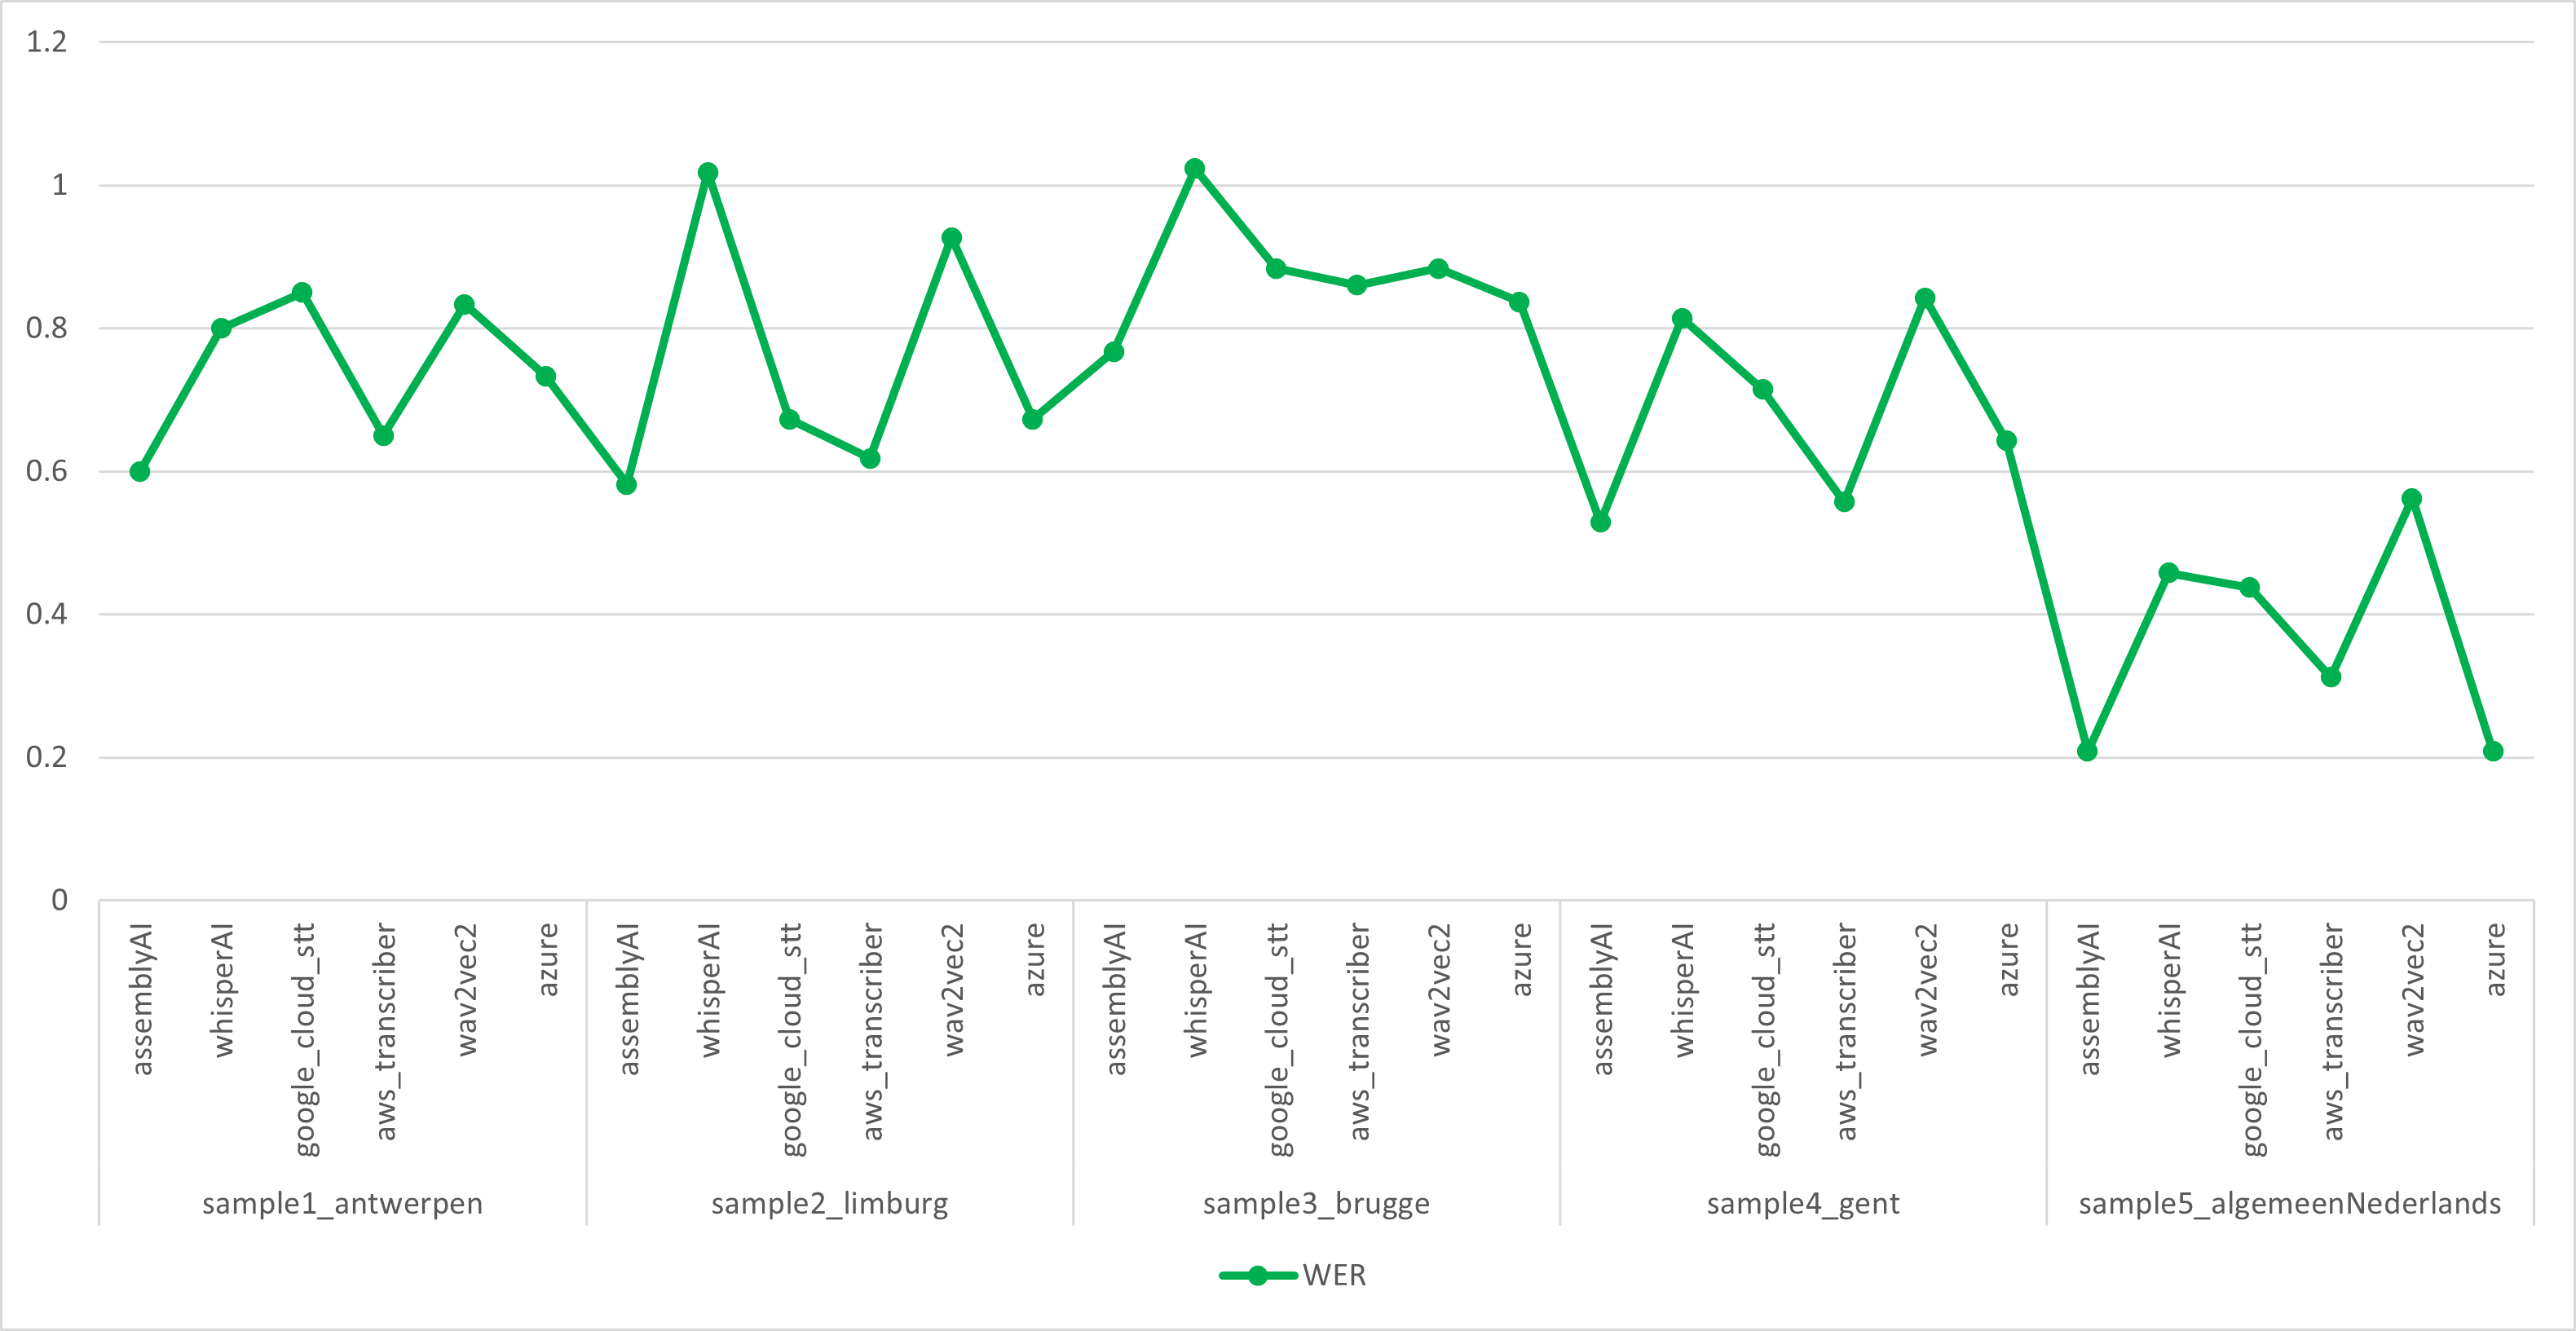
\includegraphics[width=1\textwidth]{modellenprestaties_wer.png}
    \captionsetup{justification=centering}
    \caption{Resultaat van Modellenprestaties adhv \gls{wer}}
    \label{fig:modellenprestaties_wer}
\end{figure}
\FloatBarrier

De grafiek \ref{fig:modellenprestaties_wer} toont de \gls{wer} scores van verschillende AI-modellen voor Vlaamse accenten. AssemblyAI behaalt consequent de laagste \gls{wer}-scores, wat wijst op de hoogste nauwkeurigheid.
\begin{figure}[h]
    \centering
    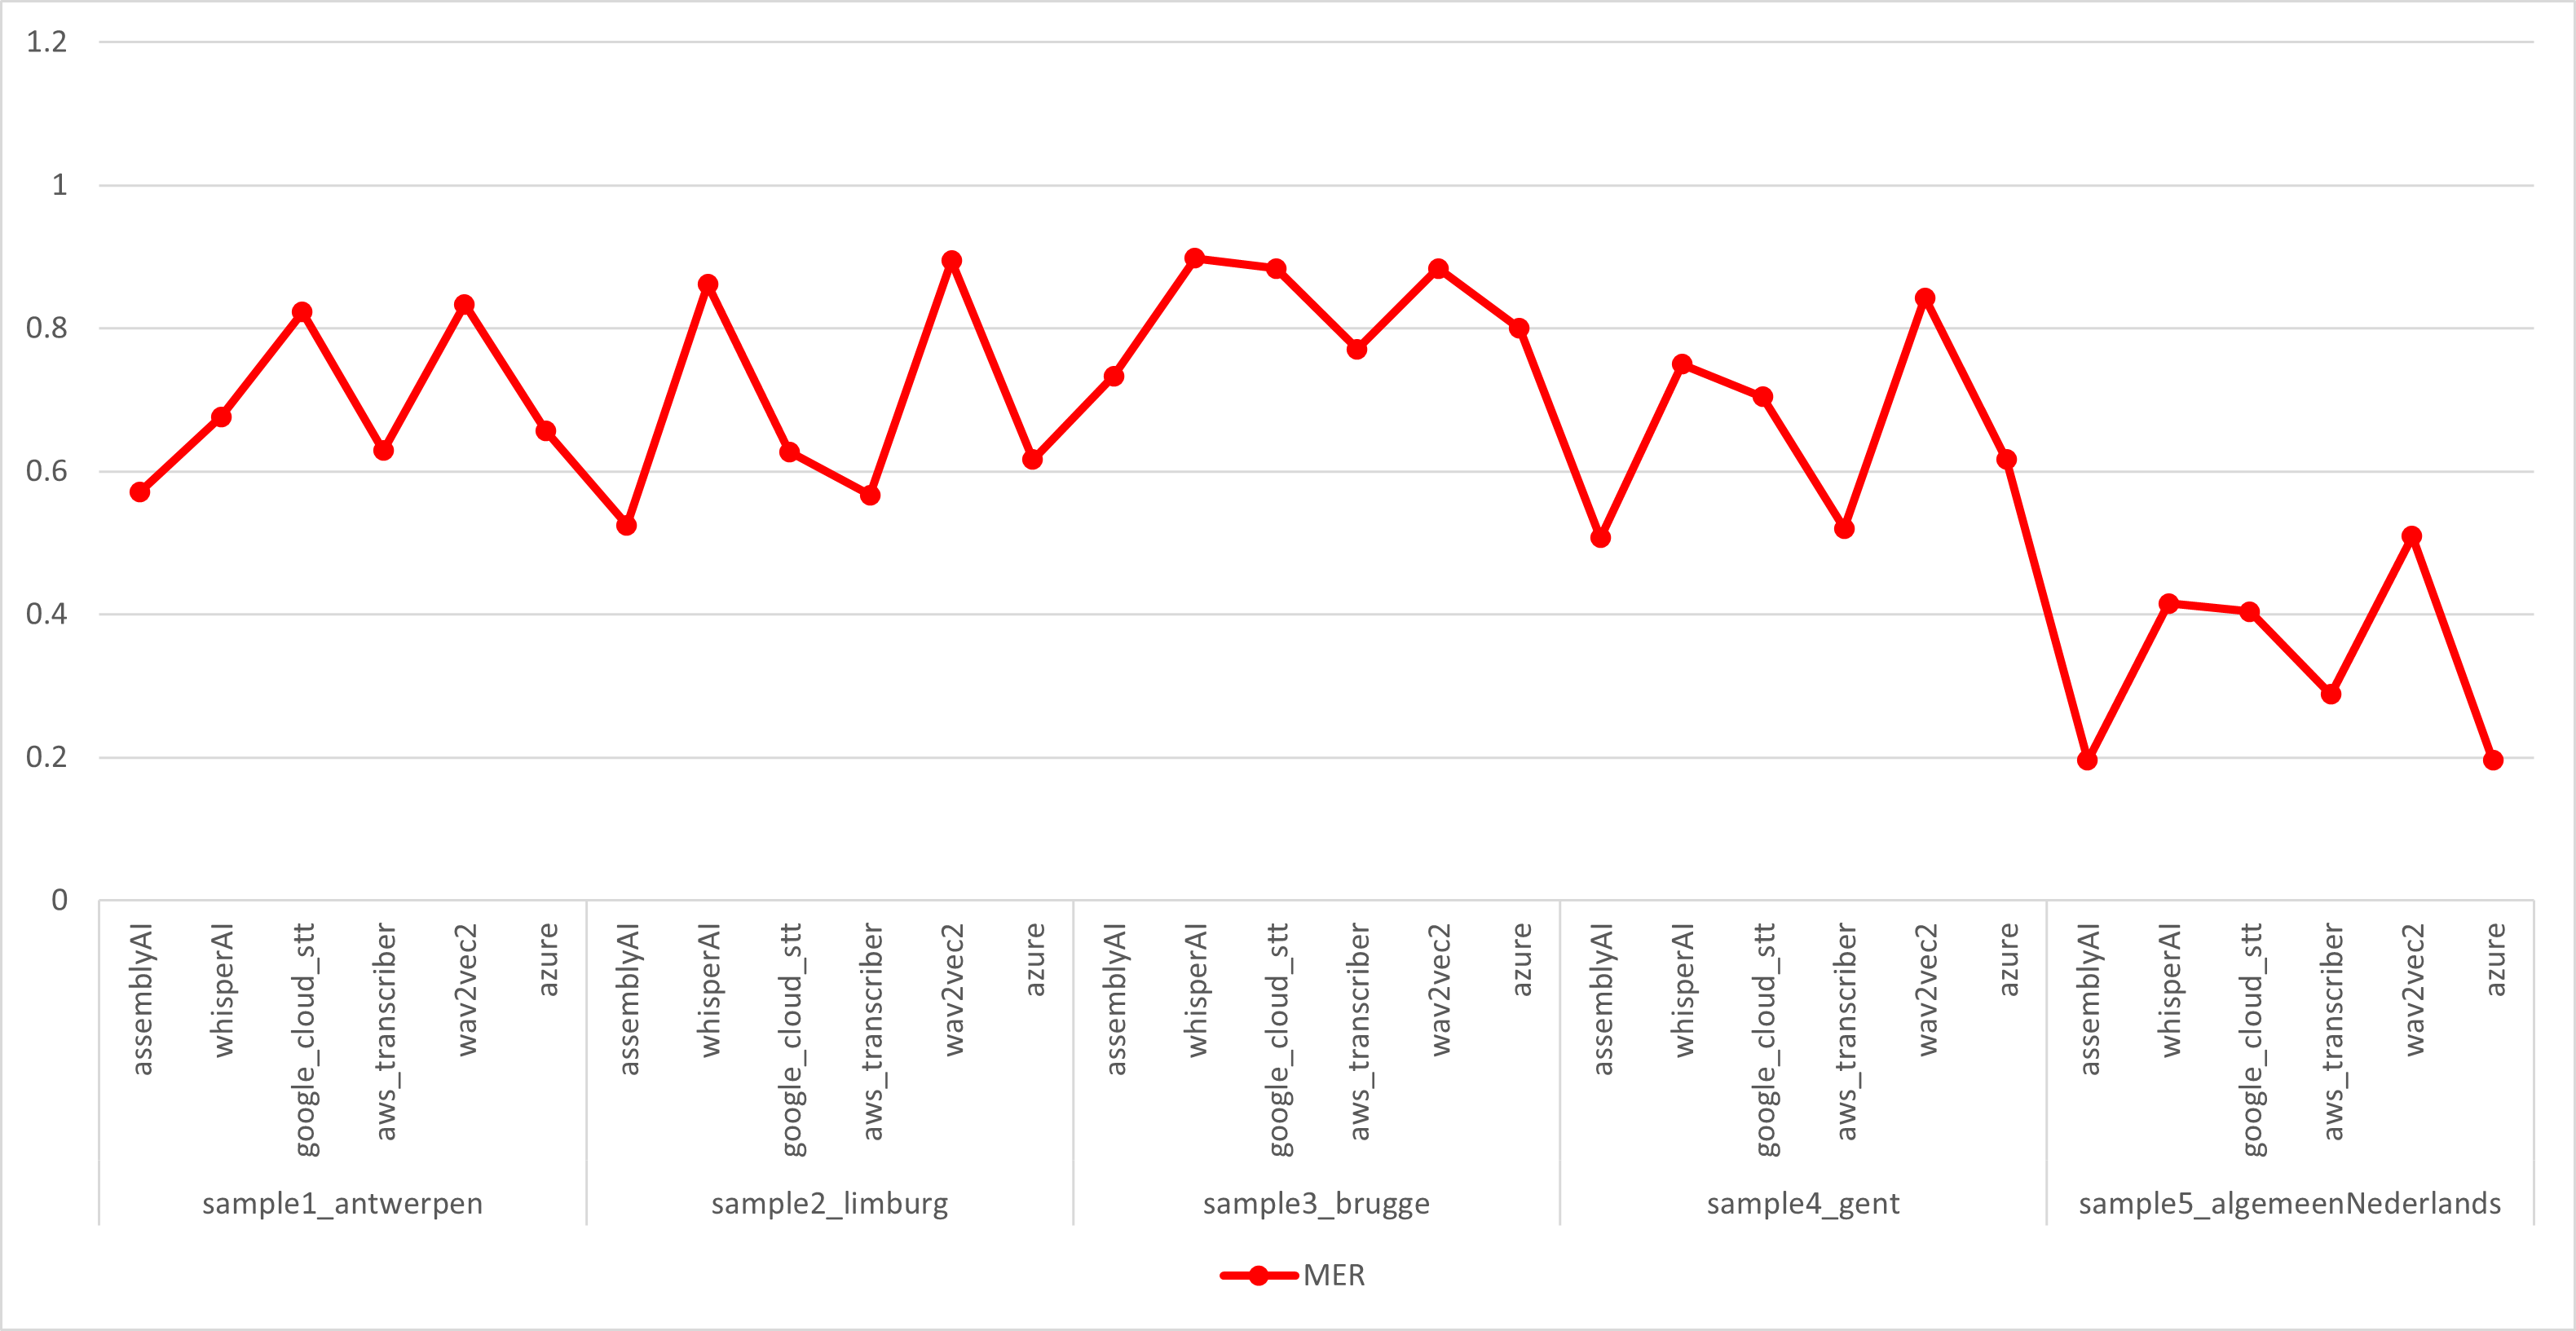
\includegraphics[width=1\textwidth]{modellenprestaties_mer.png}
    \captionsetup{justification=centering}
    \caption{Resultaat van Modellenprestaties adhv \gls{mer}}
    \label{fig:modellenprestaties_mer}
\end{figure}
\FloatBarrier

Op basis van de \gls{mer}-scores in de grafiek \ref{fig:modellenprestaties_mer} kan worden geconcludeerd dat AssemblyAI de meest betrouwbare en nauwkeurige prestaties levert bij het matchen van transcripties.

\begin{figure}[h]
    \centering
    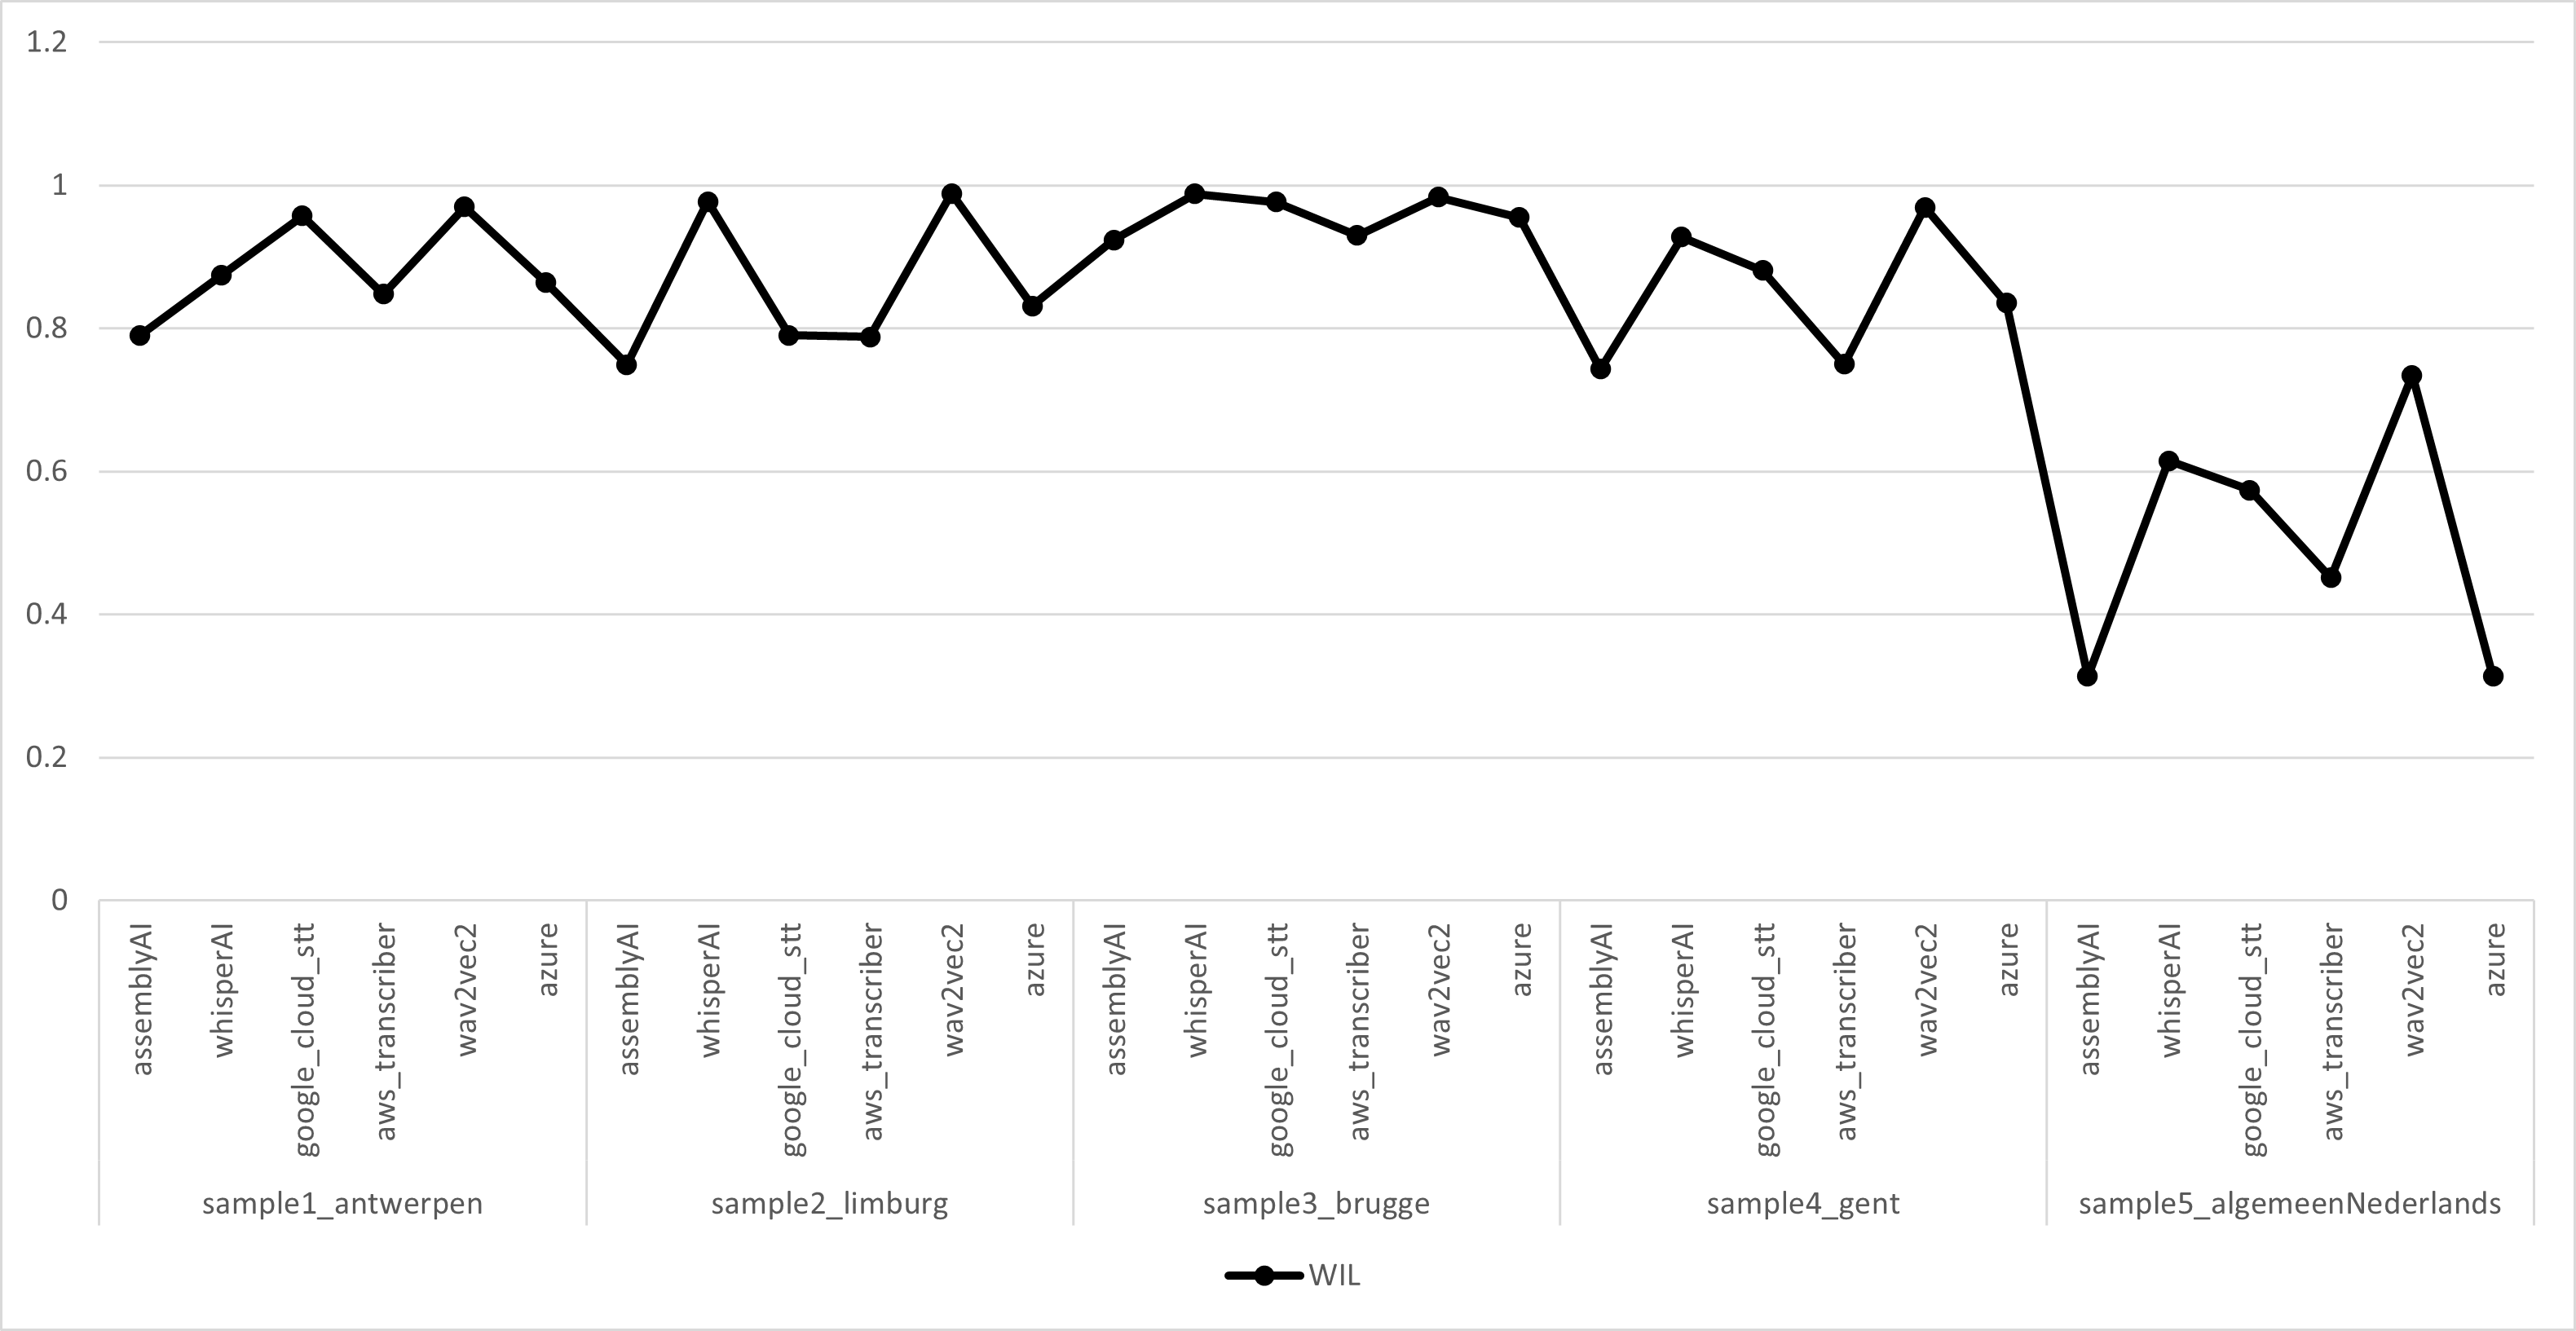
\includegraphics[width=1\textwidth]{modellenprestaties_wil.png}
    \captionsetup{justification=centering}
    \caption{Resultaat van Modellenprestaties adhv \gls{wil}}
    \label{fig:modellenprestaties_wil}
\end{figure}
\FloatBarrier
Op basis van de \gls{wil}-scores in de grafiek \ref{fig:modellenprestaties_wil} kan worden geconcludeerd dat AssemblyAI de meest betrouwbare en nauwkeurige prestaties levert bij het transcriberen van Vlaamse accenten, met het minste informatieverlies.


\begin{figure}[h]
    \centering
    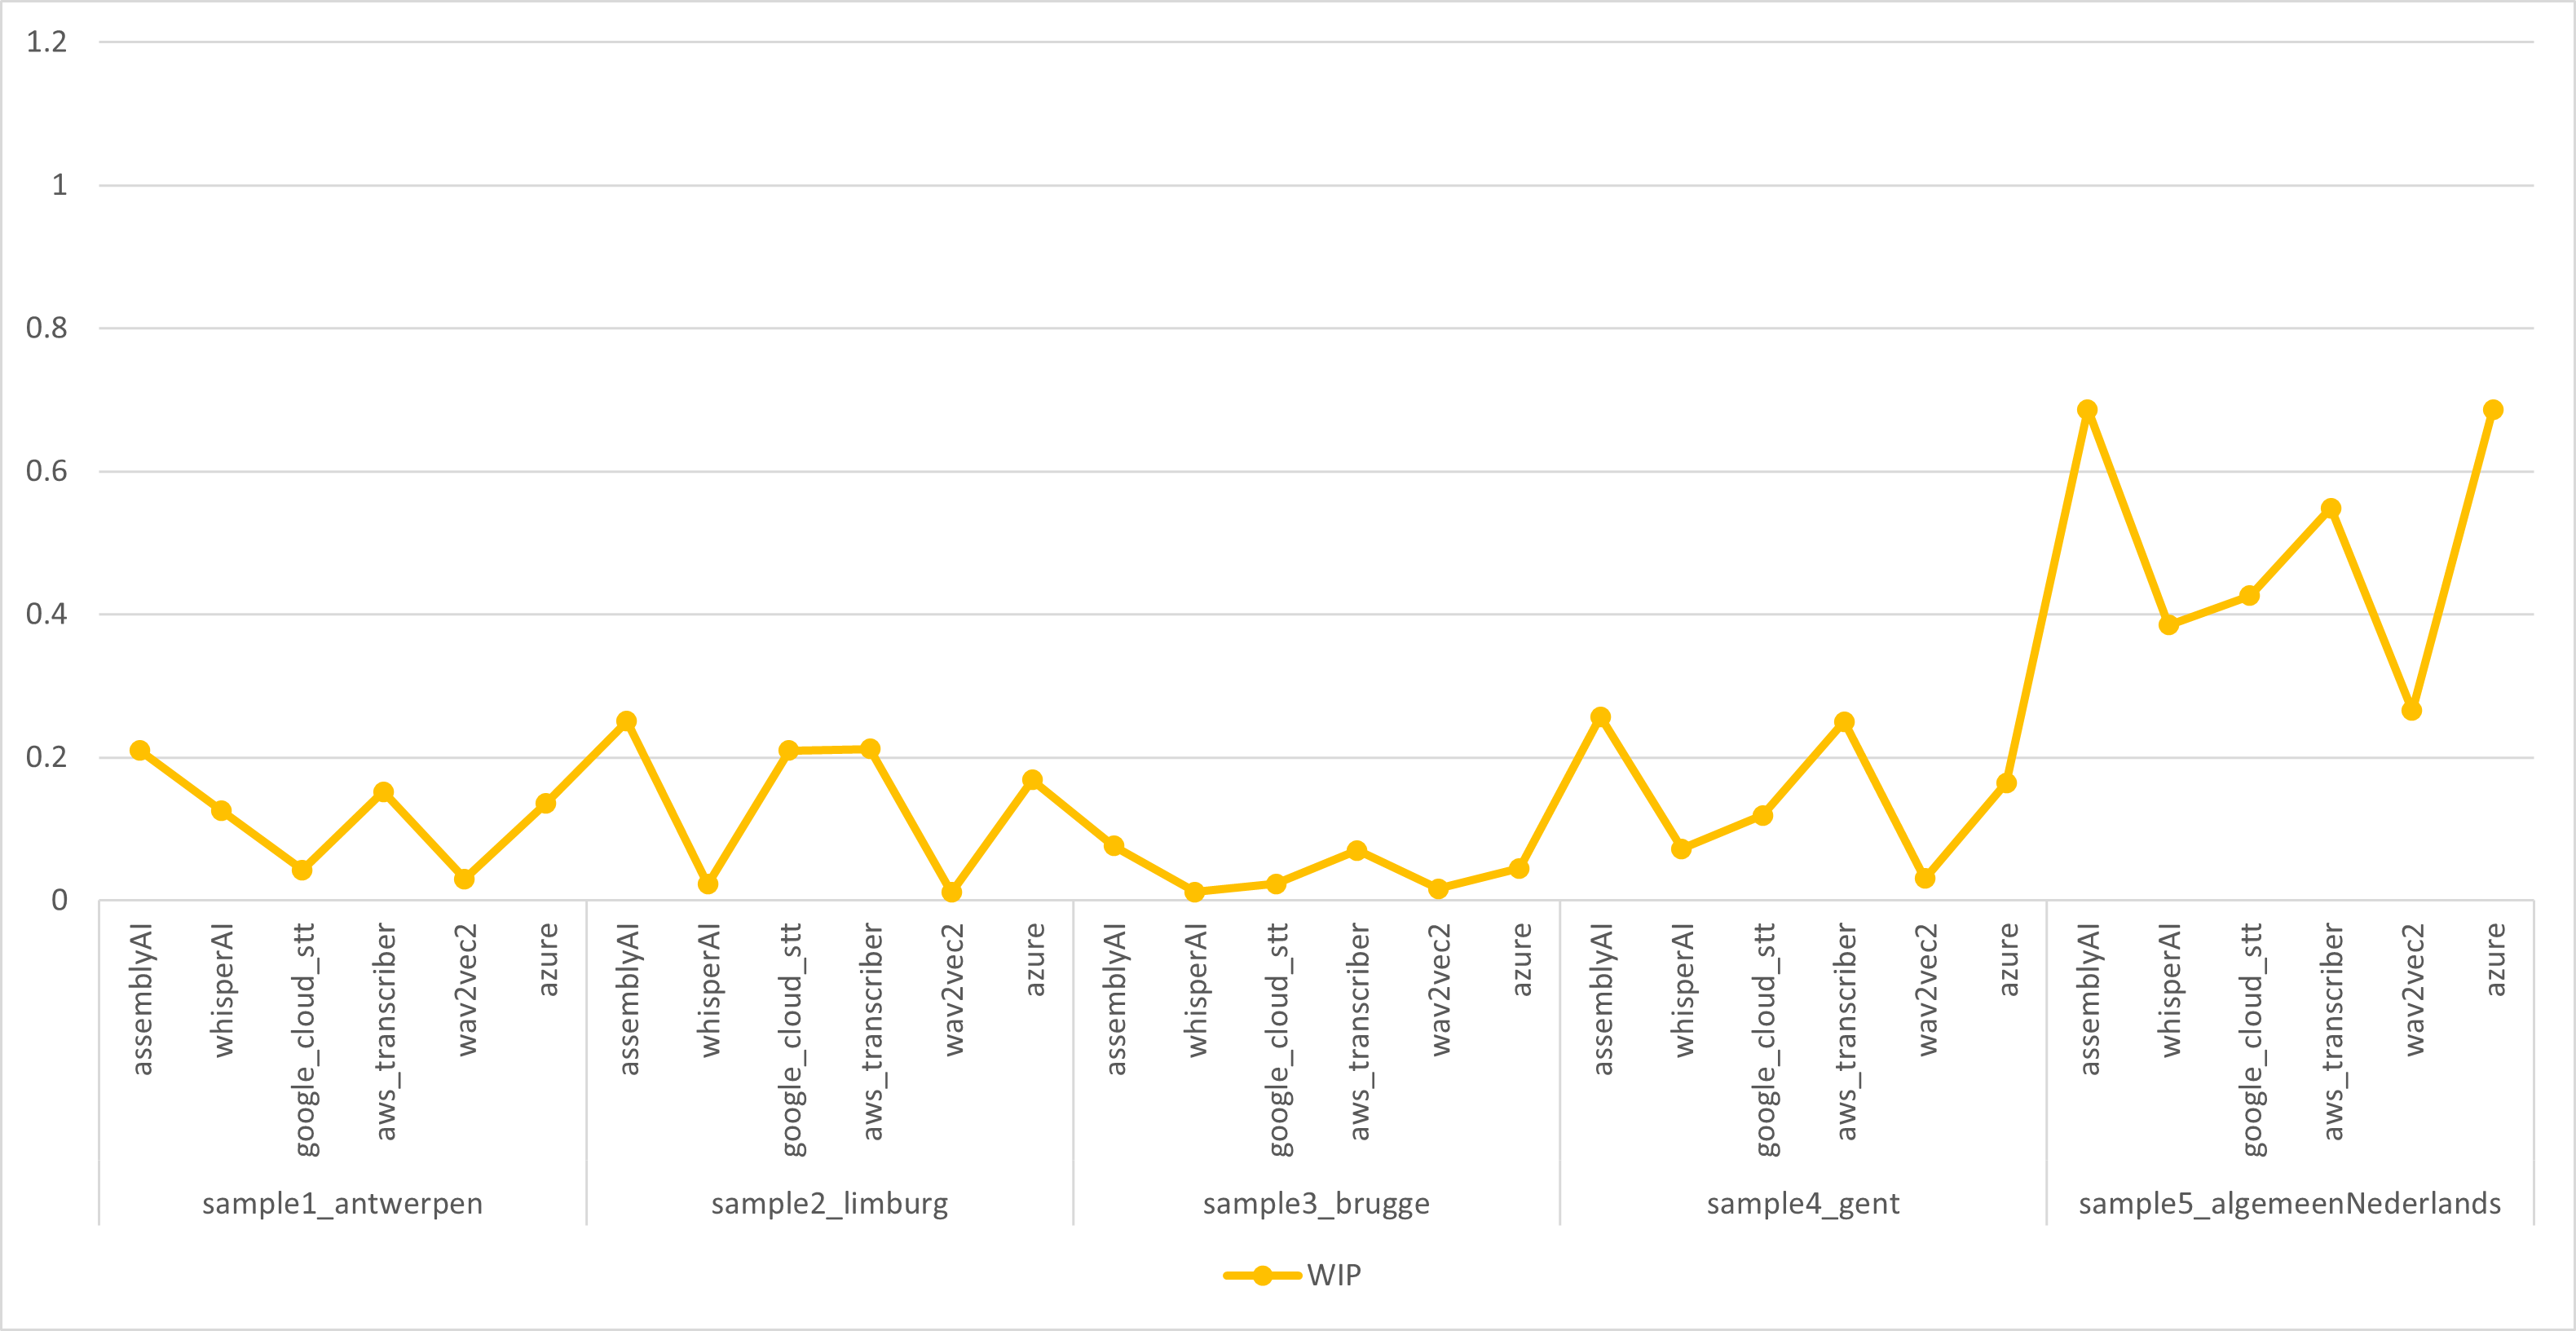
\includegraphics[width=1\textwidth]{modellenprestaties_wip.png}
    \captionsetup{justification=centering}
    \caption{Resultaat van Modellenprestaties adhv \gls{wip}}
    \label{fig:modellenprestaties_wip}
\end{figure}
\FloatBarrier
Op basis van de WIP-scores in de grafiek \ref{fig:modellenprestaties_wip} kan worden geconcludeerd dat AssemblyAI de meest betrouwbare en nauwkeurige prestaties levert bij het transcriberen van Vlaamse accenten, met het meeste behoud van informatie.

\begin{figure}[h]
    \centering
    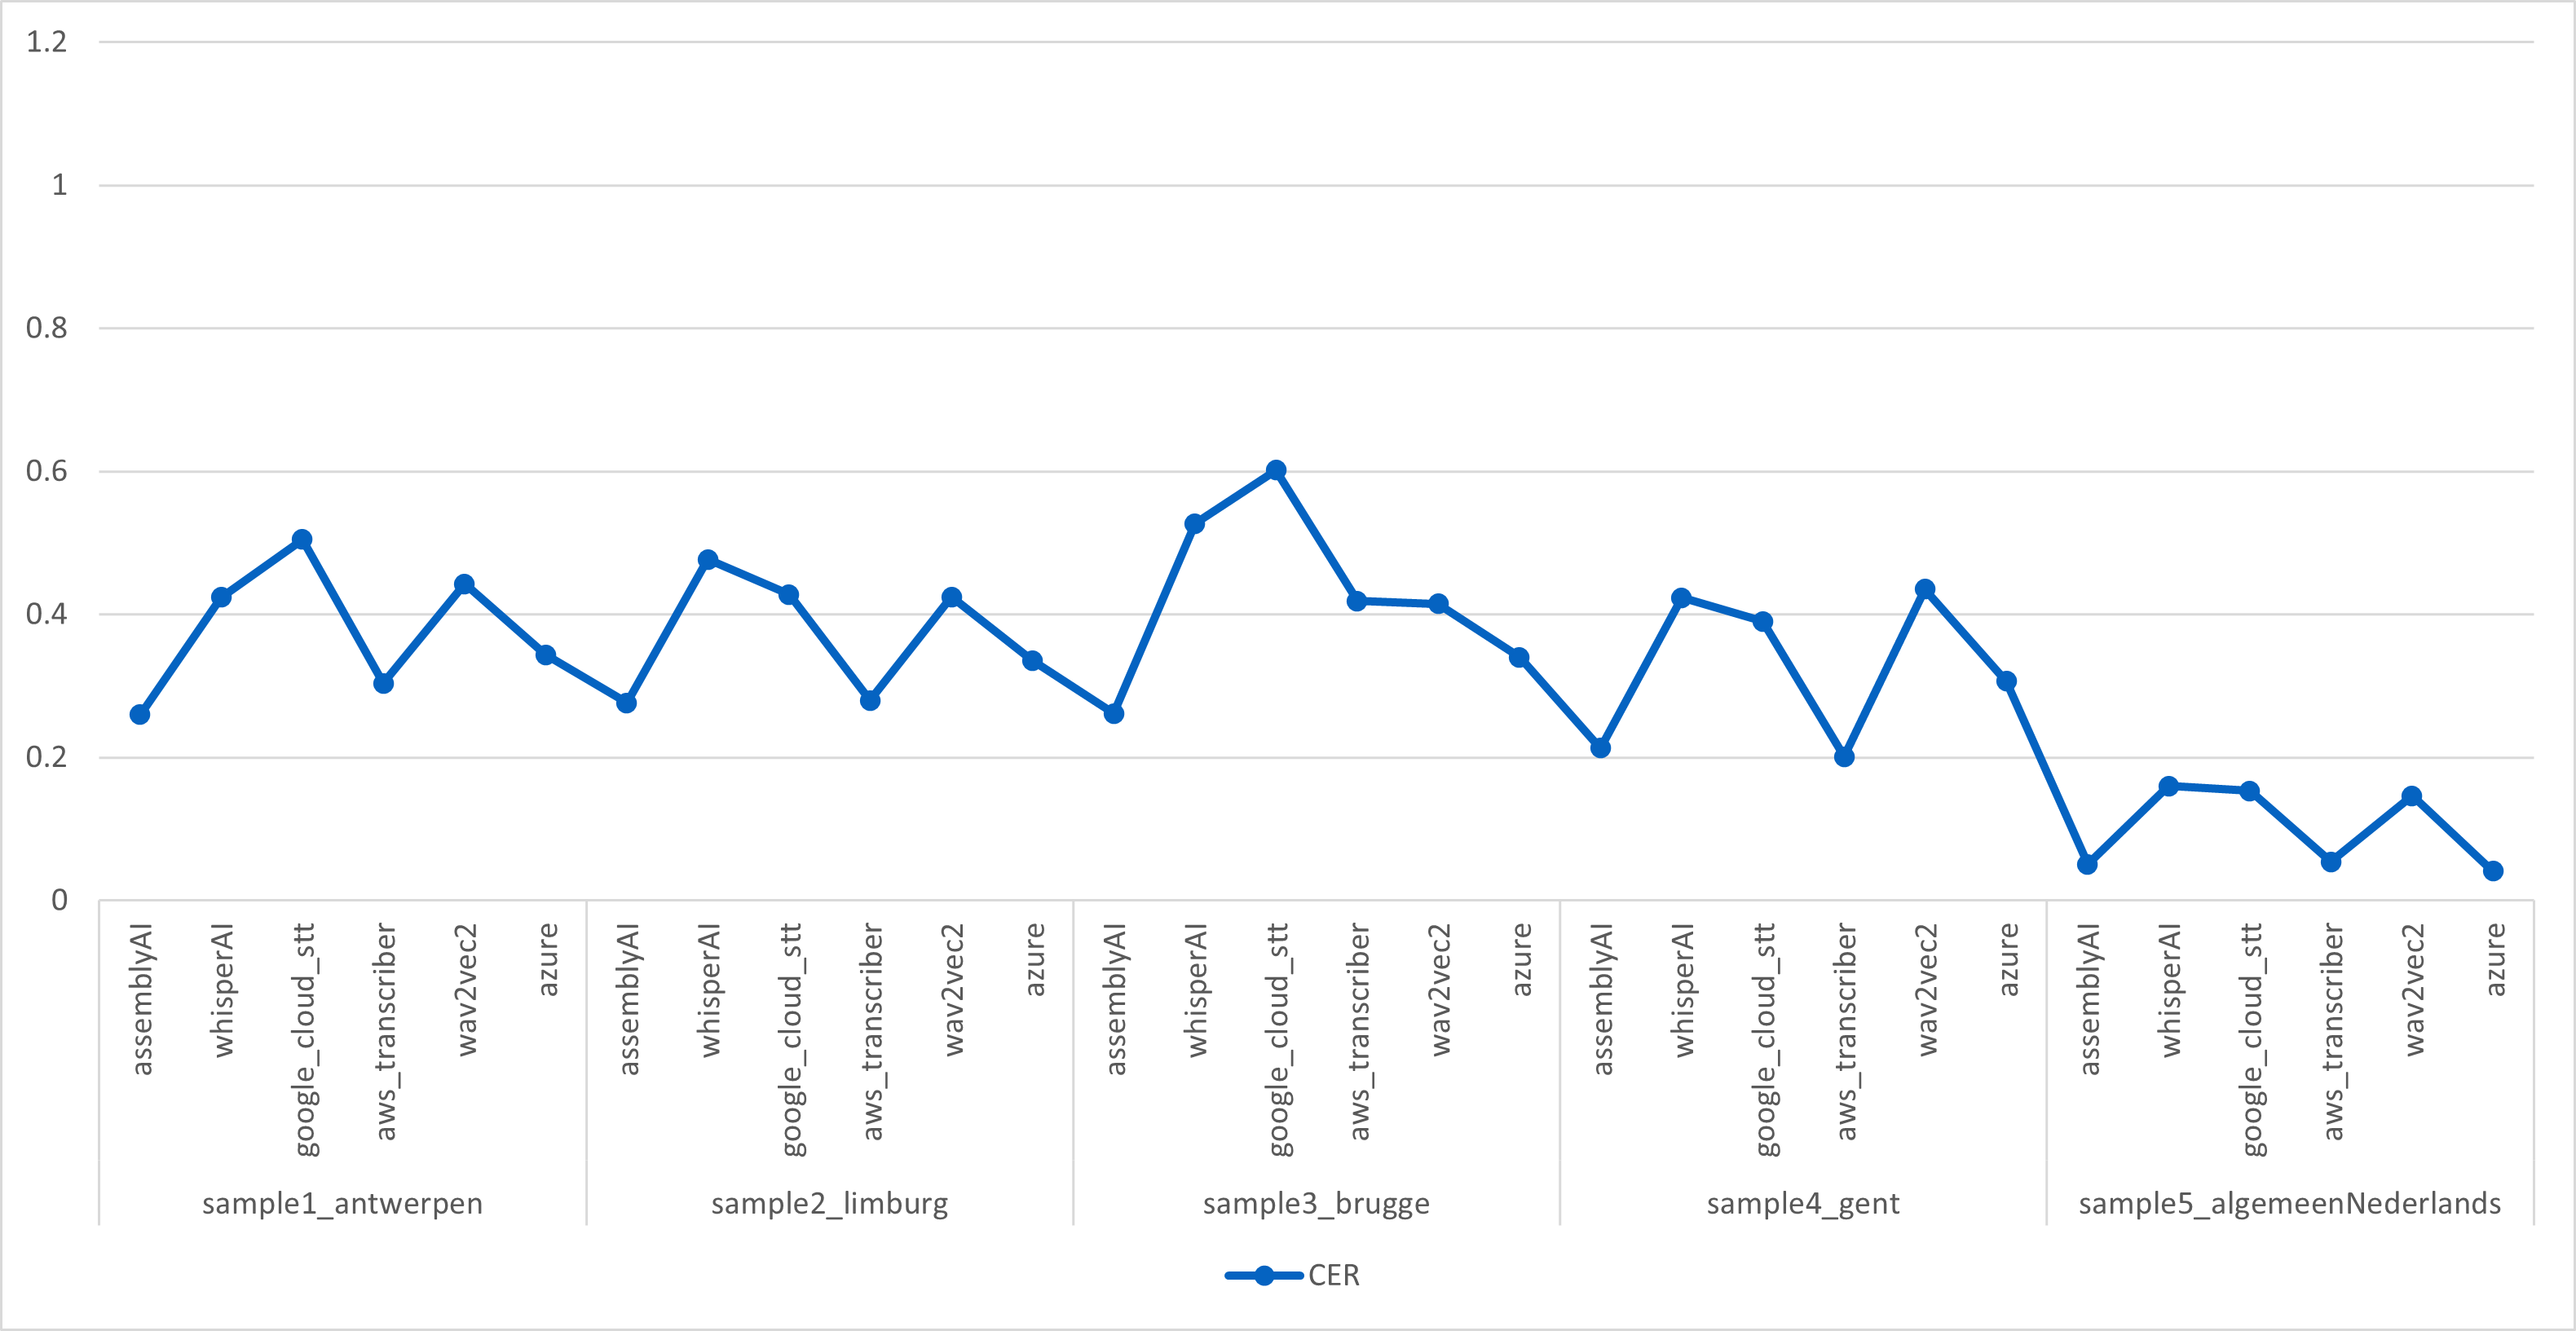
\includegraphics[width=1\textwidth]{modellenprestaties_cer.png}
    \captionsetup{justification=centering}
    \caption{Resultaat van Modellenprestaties adhv CER}
    \label{fig:modellenprestaties_cer}
\end{figure}
\FloatBarrier

De grafiek \ref{fig:modellenprestaties_cer} toont een algemeen lage \gls{cer} voor alle modellen, wat wijst op een hoge nauwkeurigheid in karakterherkenning. Het model AssemblyAI vertoont consequent lage waarden, wat de betrouwbaarheid ervan verder bevestigt.
\subsection{Conclusie}

De analyse van de prestaties van verschillende spraak-naar-tekst modellen op verschillende Nederlandse dialecten toont significante variabiliteit in de uitkomsten over de diverse metrics: \gls{wer}, \gls{mer}, \gls{wil}, \gls{wip}, en \gls{cer}.
Opvallend is dat de \gls{wer}-waarden variëren van zo laag als 0.20 voor assemblyAI in audio-opname 5 algemeenNederlands tot boven 1.0 voor whisperAI in audio-opname 2 Limburgs, wat duidt op inconsistente prestaties over de audio-opnames heen. 

WhisperAI en assemblyAI tonen significante verschillen in prestatie, met whisperAI die over het algemeen hogere ratios vertoont, wat kan wijzen op mindere efficiëntie in het omgaan met dialectische variaties vergeleken met assemblyAI.

De \gls{cer}, die de fouten op karakterbasis meet, toont een vergelijkbare trend, met lagere scores voor AssemblyAI in algemeen Nederlands maar hogere scores in meer regionaal gekleurde dialogen zoals die uit Brugge en Gent. Dit suggereert dat sommige modellen beter zijn in het algemene Nederlands dan in het verwerken van regionale accenten.

De variatie in \gls{wil} en \gls{wip} indiceert hoeveel informatie verloren gaat of behouden blijft tijdens de transcriptie, waarbij wav2vec2 consistent hoog scoort op het behoud van informatie over bijna alle audio-opnames. De resultaten suggereren dat geen enkel model universeel superieur is over alle metrieken, en dat de keuze voor een specifiek model kan afhangen van de specifieke eisen van de taak en de kenmerken van het dialect.

\section{Evaluatie Code}

In deze code \ref{lst:evaluatie_code}, wordt een tabel samengesteld die de prestaties van alle modellen weergeeft. De transcriptiegegevens, opgeslagen in een \gls{json}-bestand, worden ingeladen. Vervolgens gebruikt men de Jiwer-bibliotheek om diverse meetwaarden, zoals \gls{wer} en andere relevante metrieken, te berekenen. Na het berekenen worden deze gegevens opgeslagen in een \gls{csv}-bestand voor verdere analyse.

Daarnaast zijn er aanvullende scripts beschikbaar die de transcripties verzorgen met behulp van modellen zoals Azure, Wav2Vec2 en Whisper. Deze scripts zijn opgenomen als bijlagen en kunnen worden geraadpleegd via de volgende link \autocite{AitCheikhAhmed2024}. Voor andere modellen, namelijk AssemblyAI, Google Cloud \gls{stt} en AWS Transcriber, wordt de transcriptie gegenereerd via hun respectievelijke interfaces, waarvoor geen apart script vereist is.

\pagebreak
\begin{lstlisting}[caption={Evaluatie code}, label={lst:evaluatie_code}]
import json
import csv
from jiwer import wer, mer, wil, wip, cer

# functie om alle metrieken te berekenen adhv JWIR bib
def calculate_metrics(groundtruth, transcription):
return [
wer(groundtruth, transcription),
mer(groundtruth, transcription),
wil(groundtruth, transcription),
wip(groundtruth, transcription),
cer(groundtruth, transcription)
]

# path naar JSON DATA bestand
json_file_path = r'transcription_data.json'

# transcripties laden
with open(json_file_path, 'r') as f:
transcription_data = json.load(f)

# table headers init
table_data = [['Sample', 'Model', 'WER', 'MER', 'WIL', 'WIP', 'CER']]

# Verwerk elke input en bereken de metrieken voor de transcriptie van elke dienst.

for entry in transcription_data:
sample_name = entry['sample']

assemblyai_metrics = calculate_metrics(entry['groundtruth'], entry['assemblyai_transcription'])
whisperai_metrics = calculate_metrics(entry['groundtruth'], entry['whisperAI_transcription'])
google_cloud_metrics = calculate_metrics(entry['groundtruth'], entry['google_cloud_stt_transcription'])
aws_transcriber_metrics = calculate_metrics(entry['groundtruth'], entry['aws_transcriber_transcription'])
wav2vec2_metrics = calculate_metrics(entry['groundtruth'], entry['wav2vec2_large_xlsr_53_dutch_transcription'])
azure_metrics = calculate_metrics(entry['groundtruth'], entry['azure_transcription'])

table_data.append([sample_name, 'assemblyAI'] + assemblyai_metrics)
table_data.append(['', 'whisperAI'] + whisperai_metrics)
table_data.append(['', 'google_cloud_stt'] + google_cloud_metrics)
table_data.append(['', 'aws_transcriber'] + aws_transcriber_metrics)
table_data.append(['', 'wav2vec2'] + wav2vec2_metrics)
table_data.append(['', 'azure'] + azure_metrics)

# Schrijf de tabel output naar een CSV bestand
csv_file_path = 'transcription_metrics.csv'
with open(csv_file_path, 'w', newline='') as file:
writer = csv.writer(file)
writer.writerows(table_data)

print(f"Data has been successfully written to {csv_file_path}")

\end{lstlisting}